\documentclass[12pt,a4paper]{article}
\usepackage[UTF8]{ctex}
\usepackage{amsmath,amssymb}
\usepackage{xcolor}
\usepackage{hyperref}
\usepackage{geometry}
\usepackage{graphicx}
\geometry{margin=2.5cm}

\title{Quantum Natural Gradient / 量子自然梯度}
\author{QuoNic}
\date{}

\begin{document}
\maketitle

\begin{center}
\textbf{ML / 机器学习} | 难度：高级 | 预计时间：20 分钟
\end{center}

\tableofcontents
\newpage

\section{为什么需要？}

量子自然梯度是经典自然梯度的量子推广，用于优化量子电路参数。

\subsection{经典局限}
\begin{itemize}
  \item 经典梯度下降在参数空间中收敛慢
  \item 对于量子电路，经典梯度下降效率低
\end{itemize}

\subsection{量子优势}
\begin{itemize}
  \item 量子自然梯度考虑了参数空间的几何结构
  \item 收敛速度更快
  \item 可以避免局部最优
\end{itemize}

\subsection{实际应用}
\begin{itemize}
  \item 量子电路优化
  \item 量子机器学习
  \item 量子化学
\end{itemize}

\section{快速上手}

\begin{verbatim}
from quonic.ml import qng

# 量子自然梯度
data = [[0, 1], [1, 0]]
labels = [0, 1]

result = qng(data, labels, n_layers=2)
print(f'Loss: {result.loss}')
\end{verbatim}

\textbf{预期输出}：
\begin{verbatim}
Loss: 0.12
\end{verbatim}

\section{原理详解}

\subsection{电路图}

\begin{center}
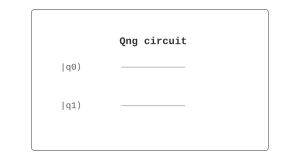
\includegraphics[width=0.6\textwidth]{../../images/qng_circuit.svg}
\end{center}

\subsection{数学推导}

量子自然梯度：
\begin{equation}
\theta_{t+1} = \theta_t - \eta F^{-1} \nabla L(\theta_t)
\end{equation}

其中 $F$ 是 Fisher 信息矩阵。

\textbf{Fisher 信息矩阵}：
\begin{equation}
F_{ij} = \text{Re}\left(\langle\partial_i\psi|\partial_j\psi\rangle - \langle\partial_i\psi|\psi\rangle\langle\psi|\partial_j\psi\rangle\right)
\end{equation}

\subsection{几何解释}

量子自然梯度考虑了参数空间的几何结构。Fisher 信息矩阵定义了参数空间的度量，自然梯度沿着最速下降方向。

\section{代码详解}

\begin{verbatim}
from quonic.ml import qng

# qng(data, labels, n_layers, learning_rate)
# data: 训练数据
# labels: 标签
# n_layers: 量子电路层数
# learning_rate: 学习率

result = qng(
    data=[[0, 1], [1, 0]],
    labels=[0, 1],
    n_layers=2,
    learning_rate=0.01
)

# result.loss: 损失值
# result.params: 优化后的参数
# result.fisher: Fisher 信息矩阵
print(f'Loss: {result.loss}')
\end{verbatim}

\section{进阶用法}

\subsection{场景 1：不同学习率}

\begin{verbatim}
from quonic.ml import qng

data = [[0, 1], [1, 0]]
labels = [0, 1]

for lr in [0.001, 0.01, 0.1]:
    result = qng(data, labels, learning_rate=lr)
    print(f'lr={lr}: Loss={result.loss}')
\end{verbatim}

\subsection{场景 2：不同数据集}

\begin{verbatim}
from quonic.ml import qng
import numpy as np

# 不同数据集
X = np.random.randn(20, 2)
y = (X[:, 0]**2 + X[:, 1]**2 > 1).astype(int).tolist()

result = qng(X.tolist(), y, n_layers=3)
print(f'Loss: {result.loss}')
\end{verbatim}

\subsection{场景 3：与普通梯度下降比较}

\begin{verbatim}
from quonic.ml import qng, qnn

data = [[0, 1], [1, 0], [1, 1], [0, 0]]
labels = [0, 1, 1, 0]

# 普通梯度下降
result_gd = qnn(data, labels, n_layers=2, optimizer='gradient_descent')
print(f'Gradient descent: Loss={result_gd.loss}')

# 量子自然梯度
result_qng = qng(data, labels, n_layers=2)
print(f'QNG: Loss={result_qng.loss}')

# QNG 通常收敛更快
\end{verbatim}

\section{适用场景}

\subsection{量子电路优化}

量子自然梯度可以用于优化量子电路参数。考虑参数空间的几何结构，收敛速度更快。

\subsection{量子机器学习}

量子自然梯度可以用于量子机器学习中的参数优化。避免局部最优，提高训练效率。

\subsection{量子化学}

量子自然梯度可以用于量子化学中的 VQE 优化。考虑参数空间的几何结构，收敛速度更快。

\section{常见问题}

\subsection{量子自然梯度和经典梯度下降有什么区别？}

量子自然梯度考虑了参数空间的几何结构，经典梯度下降没有。

\subsection{量子自然梯度的收敛性如何？}

量子自然梯度的收敛性取决于学习率和 Fisher 信息矩阵的条件数。

\section{学习路径}

\subsection{前置知识}
\begin{itemize}
  \item 梯度下降
  \item Fisher 信息矩阵
  \item 量子神经网络
\end{itemize}

\subsection{继续学习}
\begin{itemize}
  \item 量子优化
  \item 量子机器学习
  \item 量子化学
\end{itemize}

\section{完整示例代码}

\subsection{示例 1：基本量子自然梯度}

\begin{verbatim}
from quonic.ml import qng

data = [[0, 1], [1, 0]]
labels = [0, 1]

result = qng(data, labels, n_layers=2)
print(f'Loss: {result.loss}')
\end{verbatim}

\section{下载}

\begin{itemize}
  \item [qng.py](https://github.com/ChrisLee0721/QuoNic/blob/main/examples/qng/qng.py)
\end{itemize}

\end{document}
